\section{РЕЗУЛЬТАТЫ ЖАНРОВОЙ КЛАССИФИКАЦИИ}
\label{sec:genre_classification}


Для проверки значимости выделенных образов было принято решения проверить их на задаче жанровой классификации. 

В качестве исходной выборки был использован репозиторий GZTAG. Набор данных состоит из 1000 звуковых дорожек каждые по 30 секунд. Он содержит 10 жанров, каждый из которых представлен 100 треками. Все треки - это все 220-мегагерцовые Mono 16-битные аудиофайлы в формате .wav.


Для решения задачи классификации была использована библиотека scikit-learn -- бесплатная библиотека для машинного обучения с открытым исходным кодом для языка программирования Python. Все методы классификации использованы с параметрами по умолчанию. 

\subsection{AdaBoost с деревьями принятия решений}

AdaBoost zвляется мета-алгоритмом, в процессе обучения строит композицию из базовых алгоритмов обучения для улучшения их эффективности. AdaBoost является алгоритмом адаптивного бустинга в том смысле, что каждый следующий классификатор строится по объектам, которые плохо классифицируются предыдущими классификаторами.

AdaBoost вызывает слабый классификатор в цикле. После каждого вызова обновляется распределение весов, которые отвечают важности каждого из объектов обучающего множества для классификации. На каждой итерации веса каждого неверно классифицированного объекта возрастают, таким образом новый классификатор <<фокусирует своё внимание>> на этих объектах.

В качестве слабого классификаторы было использованно дерево принятие решений. Максимальное количество слабых классификаторов установлено в количестве 50. В качестве алгоритма обучения использовался алгоритм SAMME.


Как показывает рисунок \ref{fig:results:adaboost} данный классификатор плохо справляется с задачей классификации. Классифицировались фрагменты по 5 секунд с перекрытием в 0,5 секунд. Из жанров лучше всего классифицировались классическая музыка -- 70 \%, металл -- 47 \% и хипхоп -- 49 \%. 

Оценка перекрёстной проверки с десятью разбиениями -- 28 \% cо средней квадратичным отклонением 3,8 \%.  

Для задачи жанровой классификации данный метод с текущими параметрами и с теми выделенными образами для решения задачи жанровой классификации не подходит. 

\begin{figure}[h]
\centering
  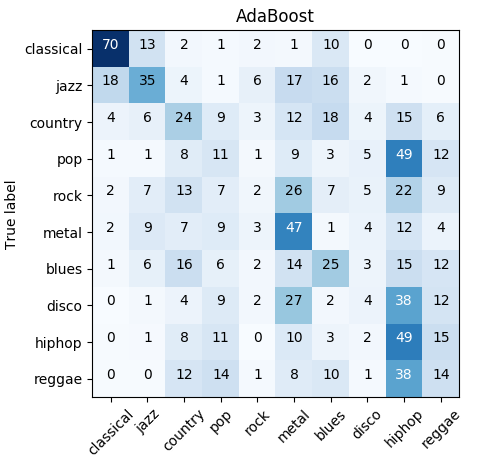
\includegraphics{AdaBoost.png}
  \caption{Матрица ошибок полученная с помощь метода классификации AdaBoost SAMME, где используется <<комитет>>  деревьев принятия решений.}
  \label{fig:results:adaboost}
\end{figure}

\subsection{Дерево принятия решений}

Деревья принятия решений - это непараметрический контролируемый метод обучения, используемый для классификации и регрессии. Цель состоит в том, чтобы создать модель, которая предсказывает значение целевой переменной путем изучения простых правил принятия решений, выведенных из данных.

В качестве алгоритма обучения используется оптимизированная версия CART. В качестве индекса неоднородности используется индекс Джини. Максимальная глубина дерева ограничена до 5 уровней.

Как показывает рисунок \ref{fig:results:DecisionTree} дерево принятия решений смогло выделить все классы, что видно по главной диагонали матрицы ошибок. Лучше всего распознались следующие жанры: классическая музыка -- 61 \%, джаз -- 56 \%, поп -- 50 \% и метал -- 58 \%. Хуже всего: диско -- 29 \%, рок -- 25 \%. 


Оценка перекрёстной проверки с десятью разбиениями -- 42 \% cо средней квадратичным отклонением 4 \%.  

\begin{figure}[h]
\centering
  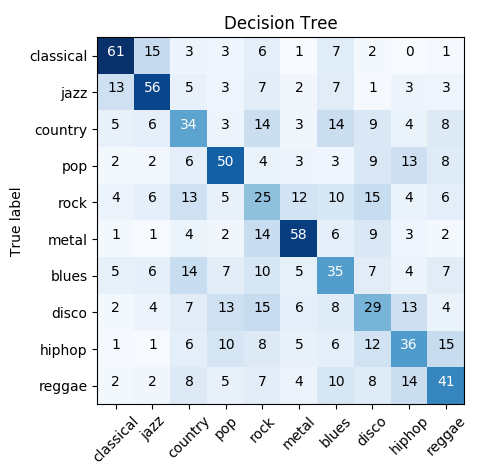
\includegraphics{DecisionTree.png}
  \caption{Матрица ошибок полученная с помощь дерева принятия решения}
  \label{fig:results:DecisionTree}
\end{figure}

При классификации всего трека использовалась интегрированная оценка по всем фрагментам. Класс трека определялся наиболее часто встречаемым предсказанным классом его фрагментов. Это улучшило результаты классификации, как можно видеть на рисунке
\ref{fig:results:DecisionTree1}. 

\begin{figure}[h]
\centering
  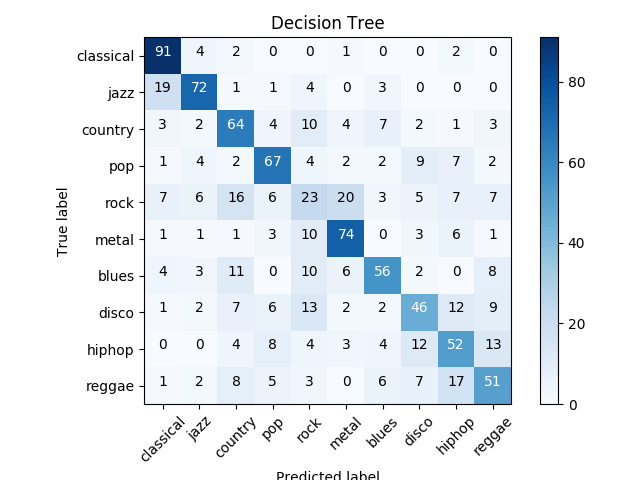
\includegraphics{DecisionTree_new1.png}
  \caption{Матрица ошибок полученная с помощь дерева принятия решения}
  \label{fig:results:DecisionTree1}
\end{figure}




\begin{figure}[h]
\centering
  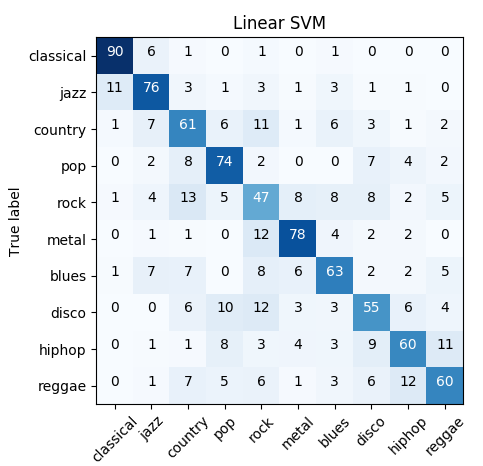
\includegraphics{LinearSVM.png}
  \caption{Матрица ошибок полученная с помощь метода опорных векторов}
  \label{fig:results:LinearSVM}
\end{figure}


\begin{figure}[h]
\centering
  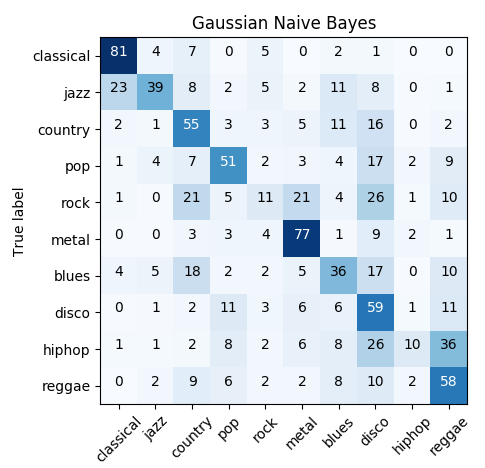
\includegraphics{NaiveBayes.png}
  \caption{Матрица ошибок полученная с помощь наивного баесовского классификатора}
  \label{fig:results:NaiveBayes}
\end{figure}

\begin{figure}[h]
\centering
  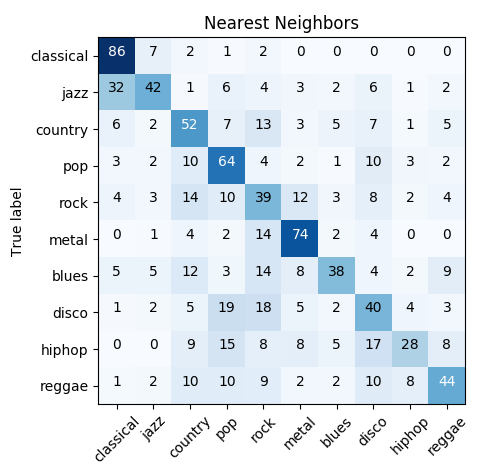
\includegraphics{NearestNeighbors.png}
  \caption{Матрица ошибок полученная с помощь метода k ближайших соседей}
  \label{fig:results:NearestNeighbors}
\end{figure}

\begin{figure}[h]
\centering
  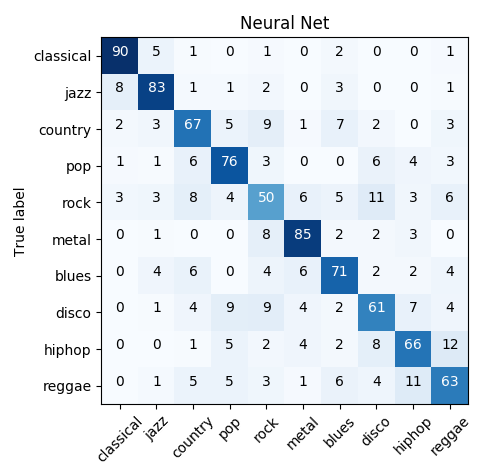
\includegraphics{NeuralNet.png}
  \caption{Матрица ошибок полученная с помощь многослойного перцептрона}
  \label{fig:results:NeuralNet}
\end{figure}


\begin{figure}[h]
\centering
  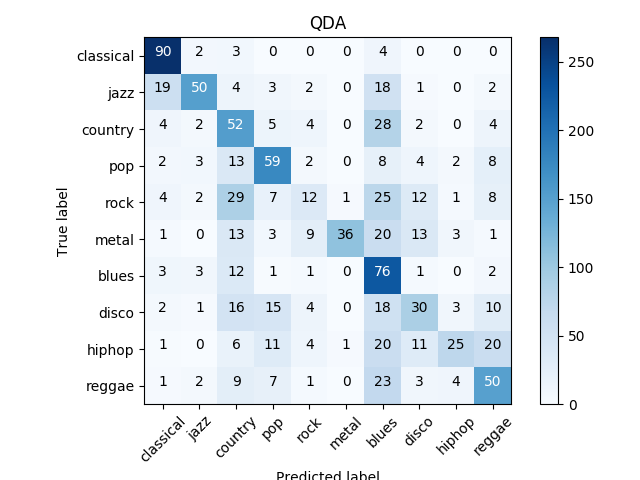
\includegraphics{QDA.png}
  \caption{Матрица ошибок полученная с помощь QDA}
  \label{fig:results:QDA}
\end{figure}


\begin{figure}[h]
\centering
  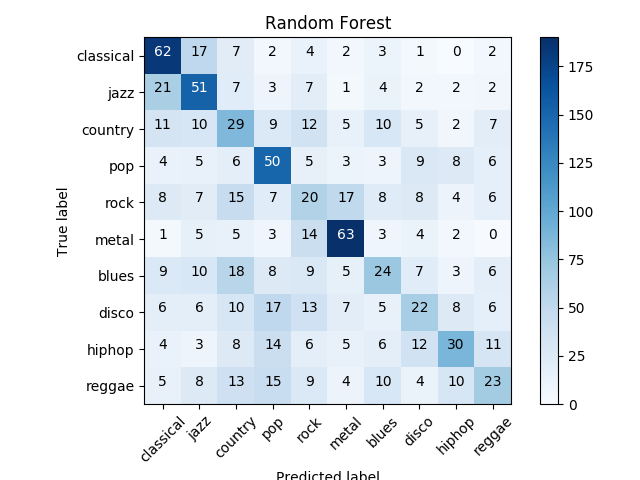
\includegraphics{RandomForest.png}
  \caption{Матрица ошибок полученная с случайного леса}
  \label{fig:results:RandomForest}
\end{figure}


В результате даже самые элементарные алгоритмы классификации показали свою эффективность, что показывает, что выделенные информационные образы значимы и могут быть использованны в системах рекомендации музыки. Все результаты сведены в таблицу
\ref{table:result}


\section{РЕЗУЛЬТАТЫ ВИЗУАЛИЗАЦИИ}
\label{sec:genre_classification}
//




